\documentclass[border=12pt]{standalone}
\usepackage{tikz,amsmath}
\usepackage[scaled]{helvet}
\renewcommand{\familydefault}{\sfdefault}
\usetikzlibrary{arrows.meta,positioning,calc,decorations.pathreplacing,patterns}
\definecolor{pro}{HTML}{1F5FA8}\definecolor{limb}{HTML}{C2410C}\definecolor{hot}{HTML}{DC2626}
\definecolor{good}{HTML}{15803D}\definecolor{ink}{HTML}{1F2937}\definecolor{quiet}{HTML}{6B7280}
\tikzset{>=Stealth,every node/.style={text=ink}}

\begin{document}
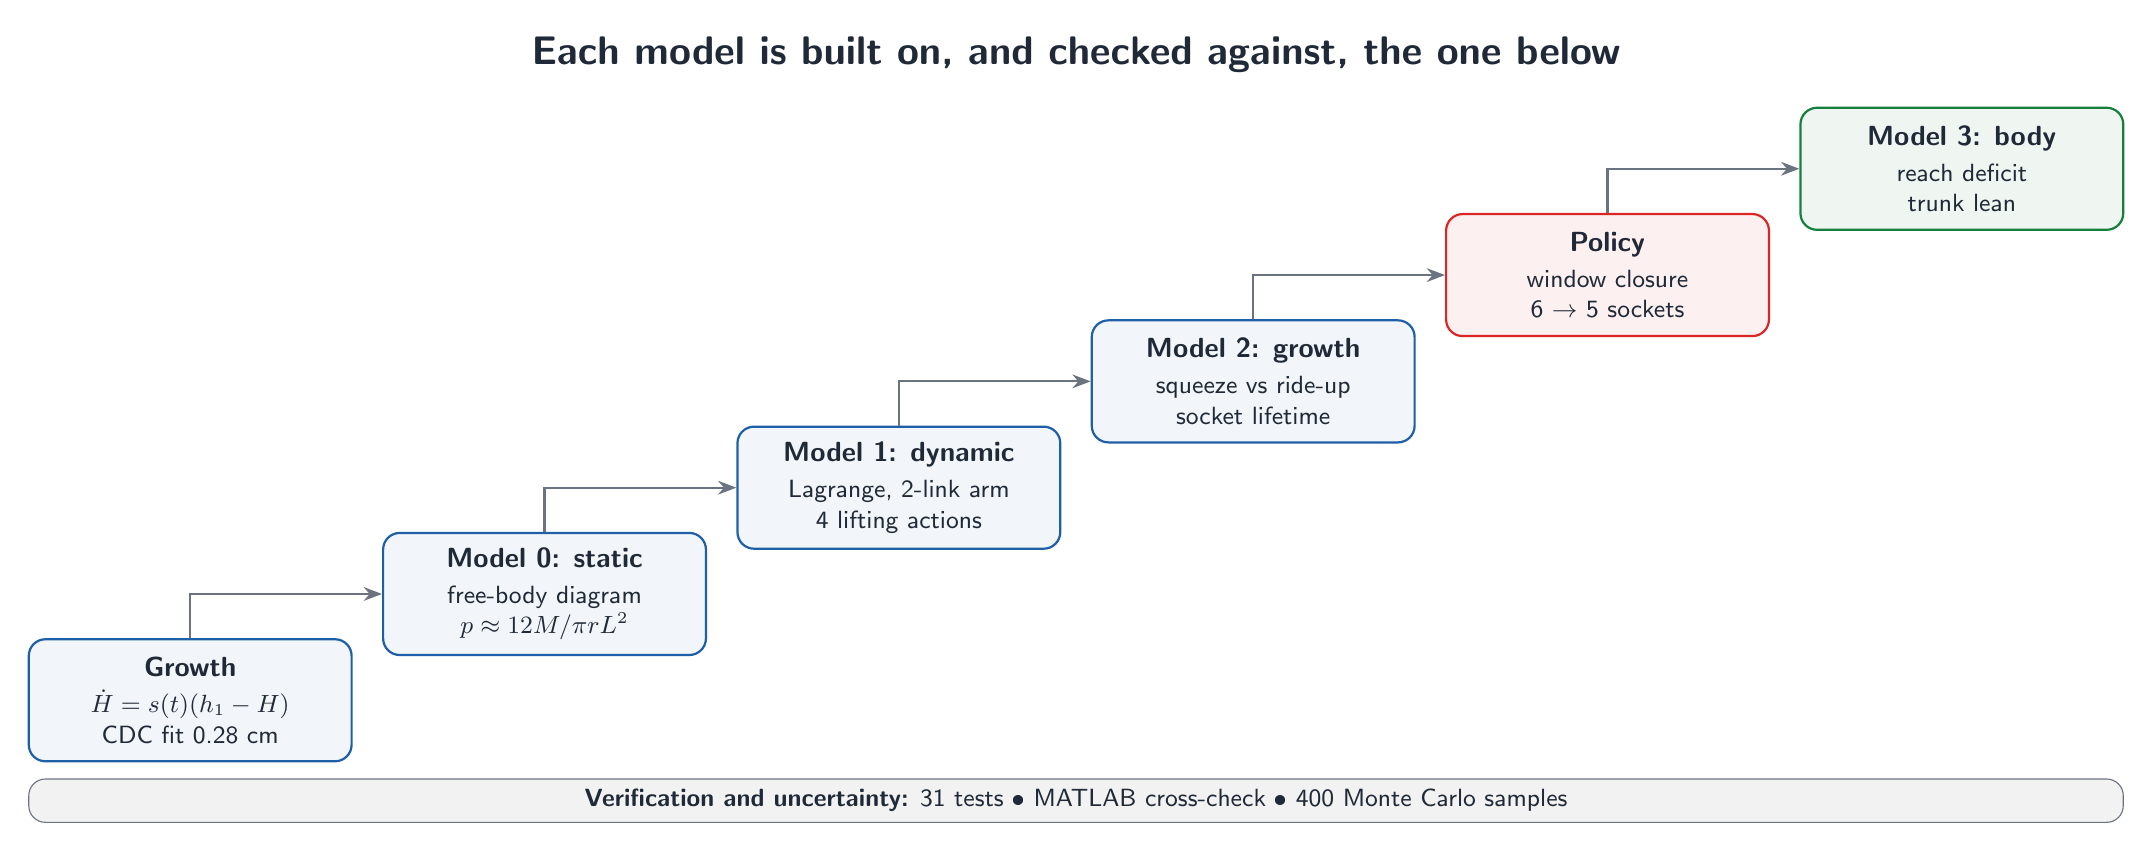
\begin{tikzpicture}[box/.style={draw=pro,thick,rounded corners=6pt,fill=pro!6,minimum width=4.1cm,minimum height=1.55cm,align=center}]
\node[font=\Large\bfseries] at (11.25,8.2) {Each model is built on, and checked against, the one below};
\node[box] (g) at (0,0) {\textbf{Growth}\\[1pt]\small $\dot H=s(t)(h_1-H)$\\[-1pt]\small CDC fit 0.28 cm};
\node[box] (m0) at (4.5,1.35) {\textbf{Model 0: static}\\[1pt]\small free-body diagram\\[-1pt]\small $p\approx 12M/\pi rL^2$};
\node[box] (m1) at (9.0,2.7) {\textbf{Model 1: dynamic}\\[1pt]\small Lagrange, 2-link arm\\[-1pt]\small 4 lifting actions};
\node[box] (m2) at (13.5,4.05) {\textbf{Model 2: growth}\\[1pt]\small squeeze vs ride-up\\[-1pt]\small socket lifetime};
\node[box,draw=hot,fill=hot!7] (p) at (18.0,5.4) {\textbf{Policy}\\[1pt]\small window closure\\[-1pt]\small 6 $\to$ 5 sockets};
\node[box,draw=good,fill=good!7] (m3) at (22.5,6.75) {\textbf{Model 3: body}\\[1pt]\small reach deficit\\[-1pt]\small trunk lean};
\foreach \a/\b in {g/m0,m0/m1,m1/m2,m2/p,p/m3} \draw[->,thick,quiet] (\a.north) |- (\b.west);
\draw[fill=gray!10,draw=quiet,rounded corners=6pt] (-2.05,-1.55) rectangle (24.55,-1.0);
\node at (11.25,-1.27) {\small\textbf{Verification and uncertainty:} 31 tests \textbullet\ MATLAB cross-check \textbullet\ 400 Monte Carlo samples};
\end{tikzpicture}
\end{document}
